%!TEX TS-program = xelatex
\documentclass{beamer}

\usepackage{HSE-theme/beamerthemeHSE} % Подгружаем тему

% инструкция по установке шрифтов: https://www.internalpointers.com/post/install-new-fonts-linux-command-line

%%% Работа с русским языком и шрифтами
\usepackage[english,russian]{babel}   % загружает пакет многоязыковой вёрстки
\usepackage{fontspec}      % подготавливает загрузку шрифтов Open Type, True Type и др.
\defaultfontfeatures{Ligatures={TeX},Renderer=Basic}  % свойства шрифтов по умолчанию
\setmainfont[Ligatures={TeX,Historic}]{Myriad Pro} %  установите шрифты Myriad Pro или (при невозможности) замените здесь на другой шрифт, который есть в системе — например, Arial
\setsansfont{Myriad Pro}  %  установите шрифты Myriad Pro или (при невозможности) замените здесь на другой шрифт, который есть в системе — например, Arial
\setmonofont{Courier New}
\uselanguage{russian}
\languagepath{russian}
\deftranslation[to=russian]{Theorem}{Теорема}
\deftranslation[to=russian]{Definition}{Определение}
\deftranslation[to=russian]{Definitions}{Определения}
\deftranslation[to=russian]{Corollary}{Следствие}
\deftranslation[to=russian]{Fact}{Факт}
\deftranslation[to=russian]{Example}{Пример}
\deftranslation[to=russian]{Examples}{Примеры}

\usepackage{animate}
\usepackage{listings}
\usepackage{multicol} 		% Несколько колонок
\usepackage{multirow}		% Несколько рядов
\usepackage{graphicx}		% images
\usepackage[justification=centering]{caption}

\graphicspath{{images/}}  	% Папка с картинками

%%% Информация об авторе и выступлении
\title[Заголовок]{3D renderer с нуля}
\subtitle{Программный проект \\ Факультет компьютерных наук}
\author[Притуляк Илья]{Притуляк Илья, БПМИ193 \texorpdfstring{\\ \scriptsize Научный руководитель: к.ф.-м.н., доцент Трушин Дмитрий Витальевич}{Lg}}
\institute[Высшая школа экономики]{Национальный исследовательский университет \\ «Высшая школа экономики» (Москва)}
\date{10 июня 2021 г.}

\begin{document}	% Начало презентации

\frame[plain]{\titlepage}	% Титульный слайд

\begin{frame}
\frametitle{Поставленные задачи}

Основная задача: написание с нуля библиотеки, решающей задачу 3D рендеринга. \pause

Сопутствующие задачи:
\begin{itemize}
	\item Изучение соответствующей литературы. \pause
	\item Краткое изложение всей необходимой теории. \pause
	\item Тестирование написанного кода на производительность. \pause
	\item Написание сопроводительной документации. \pause
\end{itemize}

Репозиторий проекта: \url{https://github.com/stabmind/3D-renderer}

\end{frame}

\begin{frame}
\frametitle{Pipeline}

Этапы рендеринга:
\begin{itemize}
	\item Модельное преобразование. \pause
	\item Видовое преобразование. \pause
	\item Клиппинг. \pause
	\item Перспективное преобразование. \pause
	\item Растеризация.
\end{itemize}
\end{frame}

\begin{frame}
\frametitle{Архитектура}

Сторонние библиотеки: SFML, Eigen. \pause

Библиотечные классы:
\begin{itemize}
	\item Triangle \pause
 	\item World \pause
 	\item Camera \pause
 	\item Screen \pause
 	\item Renderer \pause
 	\item Application
\end{itemize}
\end{frame}

\begin{frame}[fragile]
\frametitle{Архитектура}

\lstset{language=C++,
        basicstyle=\ttfamily,
        keywordstyle=\color{red}\ttfamily,
        commentstyle=\color{gray}\ttfamily
}
\begin{lstlisting}
#include "application.h"

// Application contains:
// World, Camera, Screen, Renderer

int main() {
    /* application preparing */
    app.RunInteractiveScene();
    return 0;
}
\end{lstlisting}
\end{frame}

\begin{frame}[fragile]
\frametitle{Архитектура}

\lstset{language=C++,
        basicstyle=\ttfamily,
        keywordstyle=\color{red}\ttfamily,
        commentstyle=\color{gray}\ttfamily}

\begin{lstlisting}
void RunInteractiveScene() {
    InitWindow();
    while (window is open) {
        /* commands processing  */
        renderer.Render(world, camera, screen);
        Draw();
    }
}
\end{lstlisting}
\end{frame}

\begin{frame}
\frametitle{Примеры работы}

\begin{figure}
    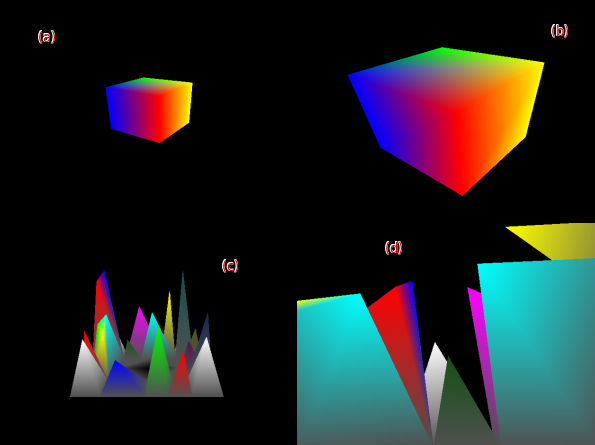
\includegraphics[scale=0.3]{rendered models.png}
    \caption*{Модели куба и гор с разных ракурсов.}
\end{figure}
\end{frame}

\begin{frame}
\frametitle{Результаты тестирования}

\begin{center}
	\begin{tabular}{|c|c|c|c|c|c|c|} \hline
		\multirow{3}{*}{Разрешение}
		& \multicolumn{6}{|c|}{FPS} \\ \cline{2-7}
		& \multicolumn{3}{|c|}{Куб} & \multicolumn{3}{|c|}{Горы} \\ \cline{2-7}
		& Вдали & Вблизи & Min & Вдали & Вблизи & Min \\ \hline
		$640 \times 480$ & 70 & 60 & 21 & 60 & 38 & 13 \\ \hline
		$1280 \times 720$ & 28 & 21 & 11 & 25 & 14 & 7 \\ \hline
		$1920 \times 1080$ & 10 & 8 & 5 & 10 & 6 & 3 \\ \hline
	\end{tabular}
\end{center}

Процессор: Intel(R) Core(TM) i3-6100U CPU @ 2.30GHz.

\end{frame}

\begin{frame}
\frametitle{Итог}

Достигнутые цели:
\begin{itemize}
	\item Реализован 3D renderer с поддержкой интерактивного режима. \pause
	\item Изложена вся необходимая для понимания темы теория, за исключением математических доказательств. \pause
	\item Написанный код протестирован на производительность. \pause
	\item Написана сопроводительная документация.
\end{itemize}
\end{frame}

\end{document}
